\chapter{Конструкторская часть}

\section{Диаграммы IDEF0}

На рисунках \ref{fig:idef0_0} и \ref{fig:idef0_1} представлены диаграммы в нотации IDEF0, отражающие процесс мониторинга приоритетов, времени непрерывной работы, простоя и блокировки процессов.

\begin{figure}[H]
	\centering
	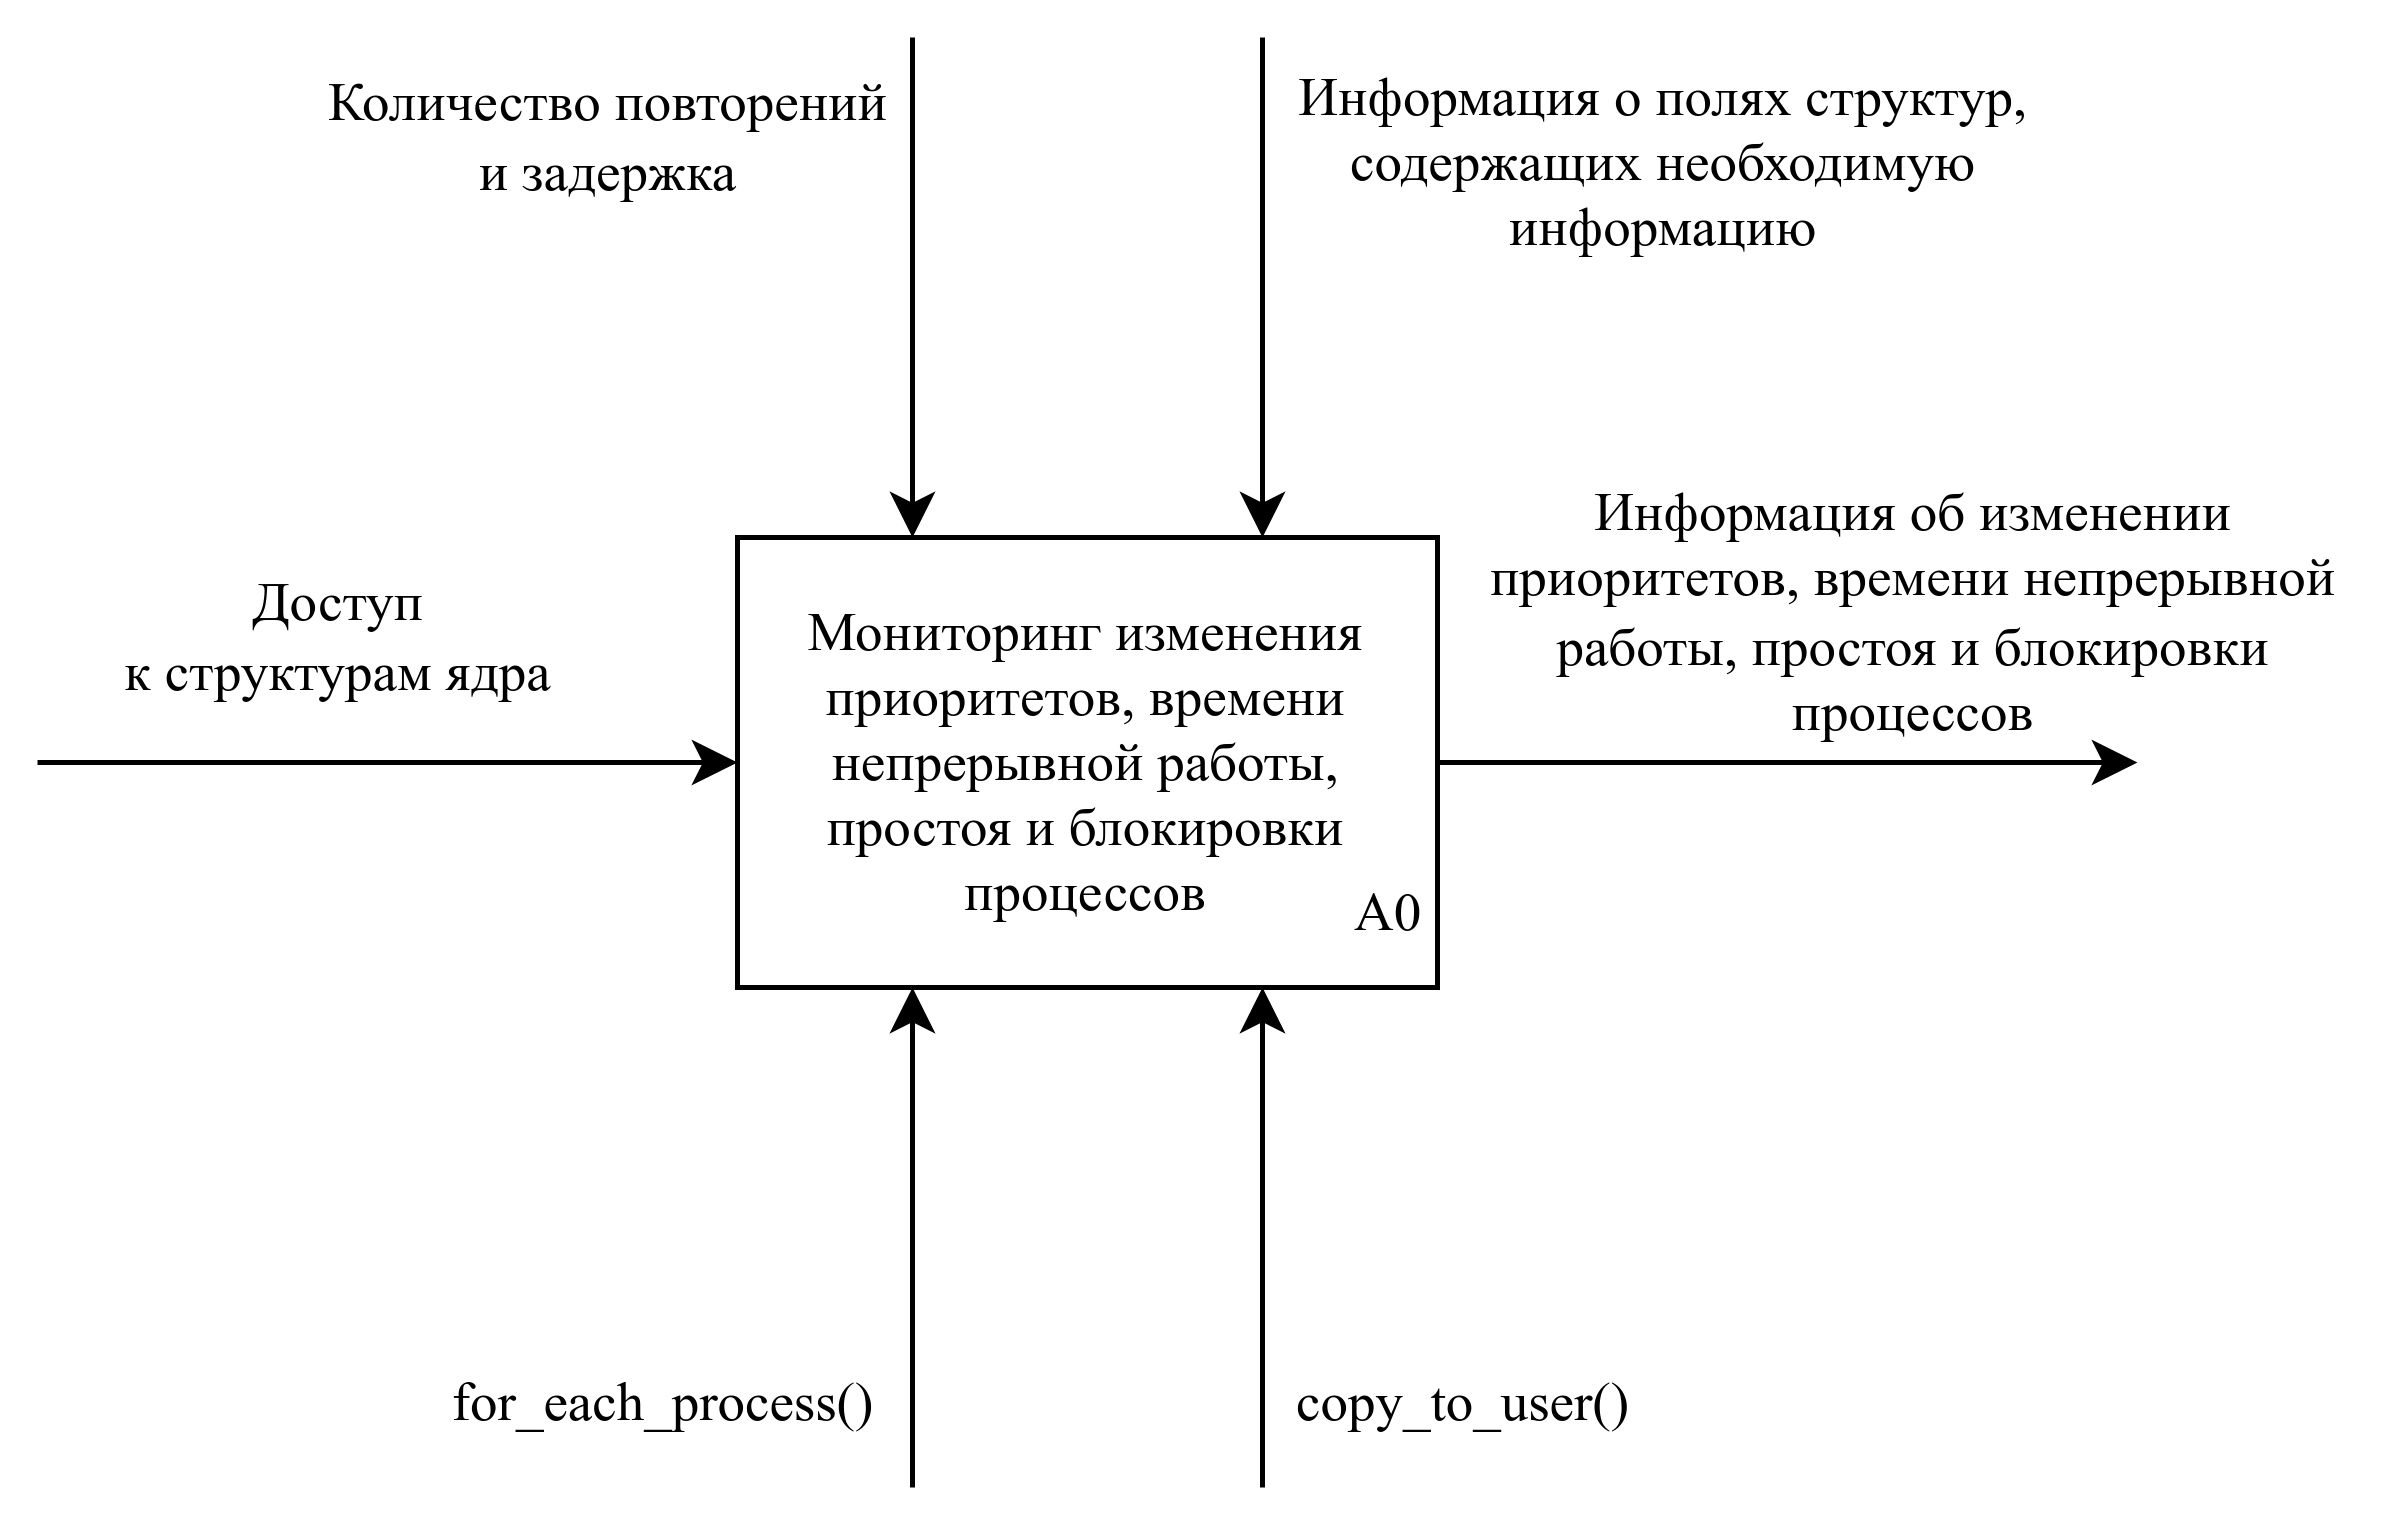
\includegraphics[width=\textwidth]{assets/idef0_a0.png}
	\caption{Диаграмма IDEF0, нулевой уровень}
	\label{fig:idef0_0}
\end{figure}

\begin{figure}[H]
	\centering
	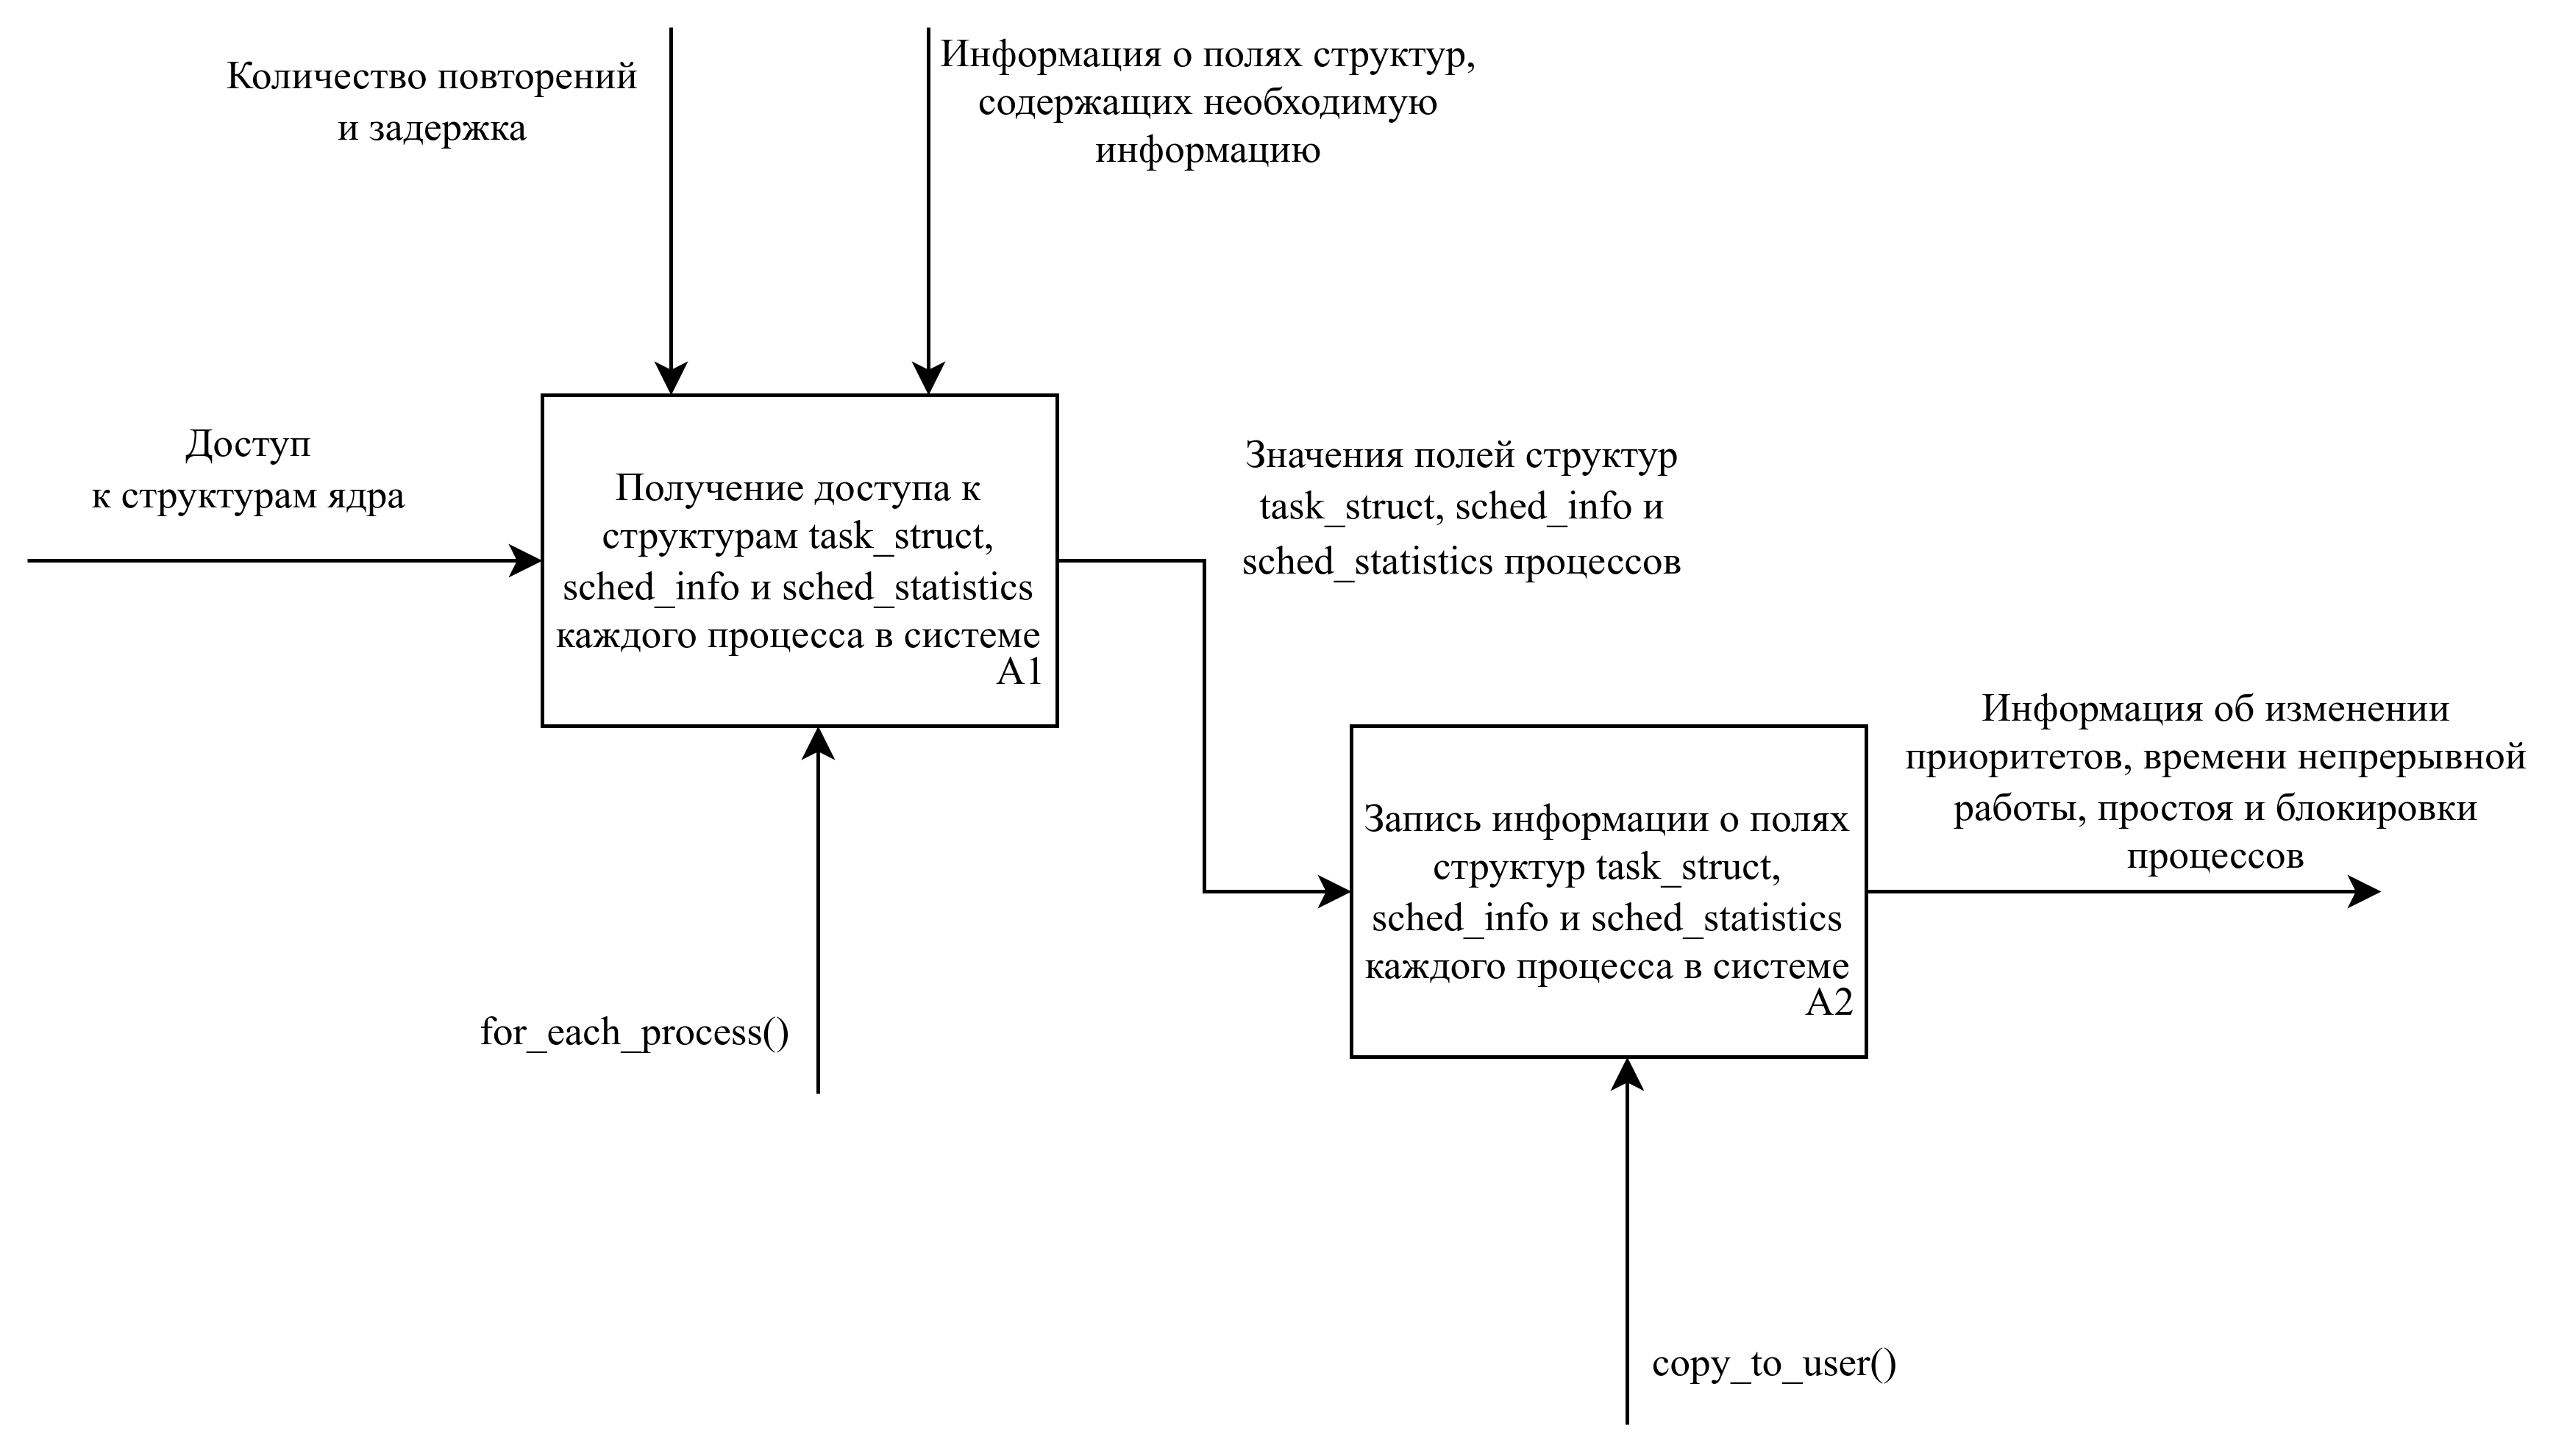
\includegraphics[width=\textwidth]{assets/idef0_a1.png}
	\caption{Диаграмма IDEF0, первый уровень}
	\label{fig:idef0_1}
\end{figure}

\section{Алгоритмы определения и сохранения приоритетов, времени непрерывной работы, простоя и блокировки процессов}

На рисунках \ref{fig:kernel} и \ref{fig:log} представлены алгоритмы определения и сохранения приоритетов, времени непрерывной работы, простоя и блокировки процессов.

\begin{figure}[H]
	\centering
	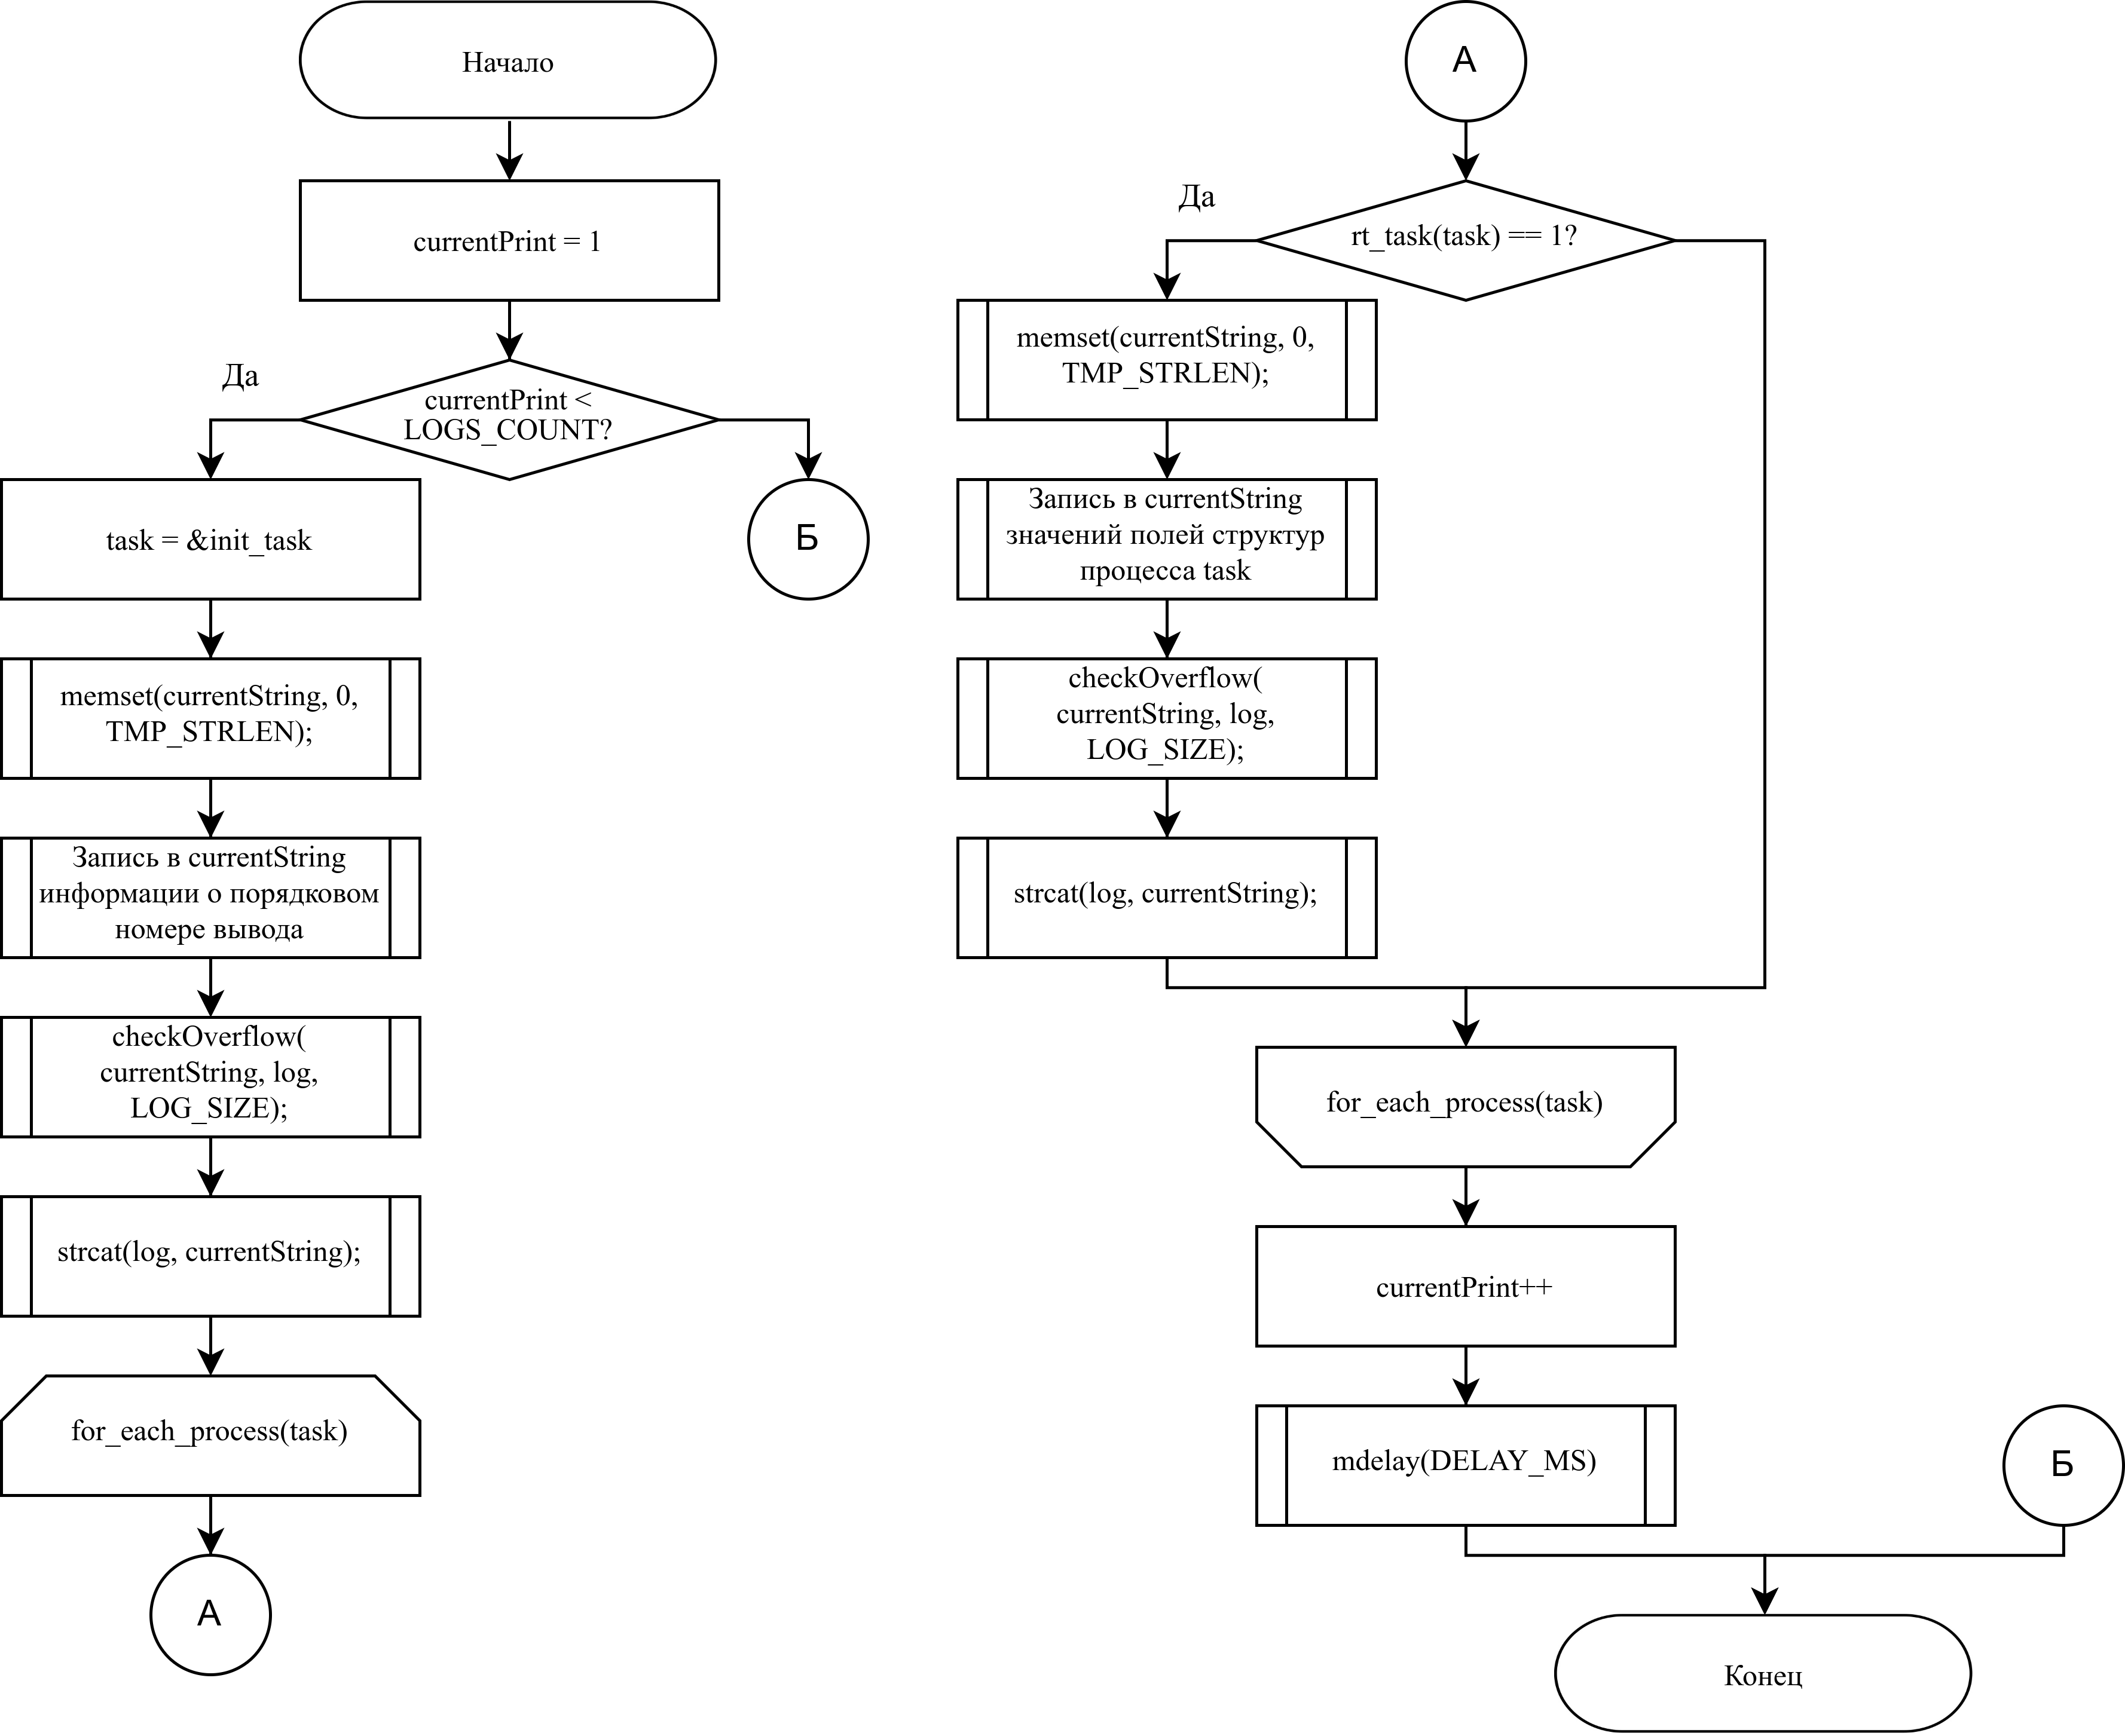
\includegraphics[width=\textwidth]{assets/kernel.png}
	\caption{Алгоритм определения приоритетов, времени непрерывной работы, простоя и блокировки процессов}
	\label{fig:kernel}
\end{figure}

\begin{figure}[H]
	\centering
	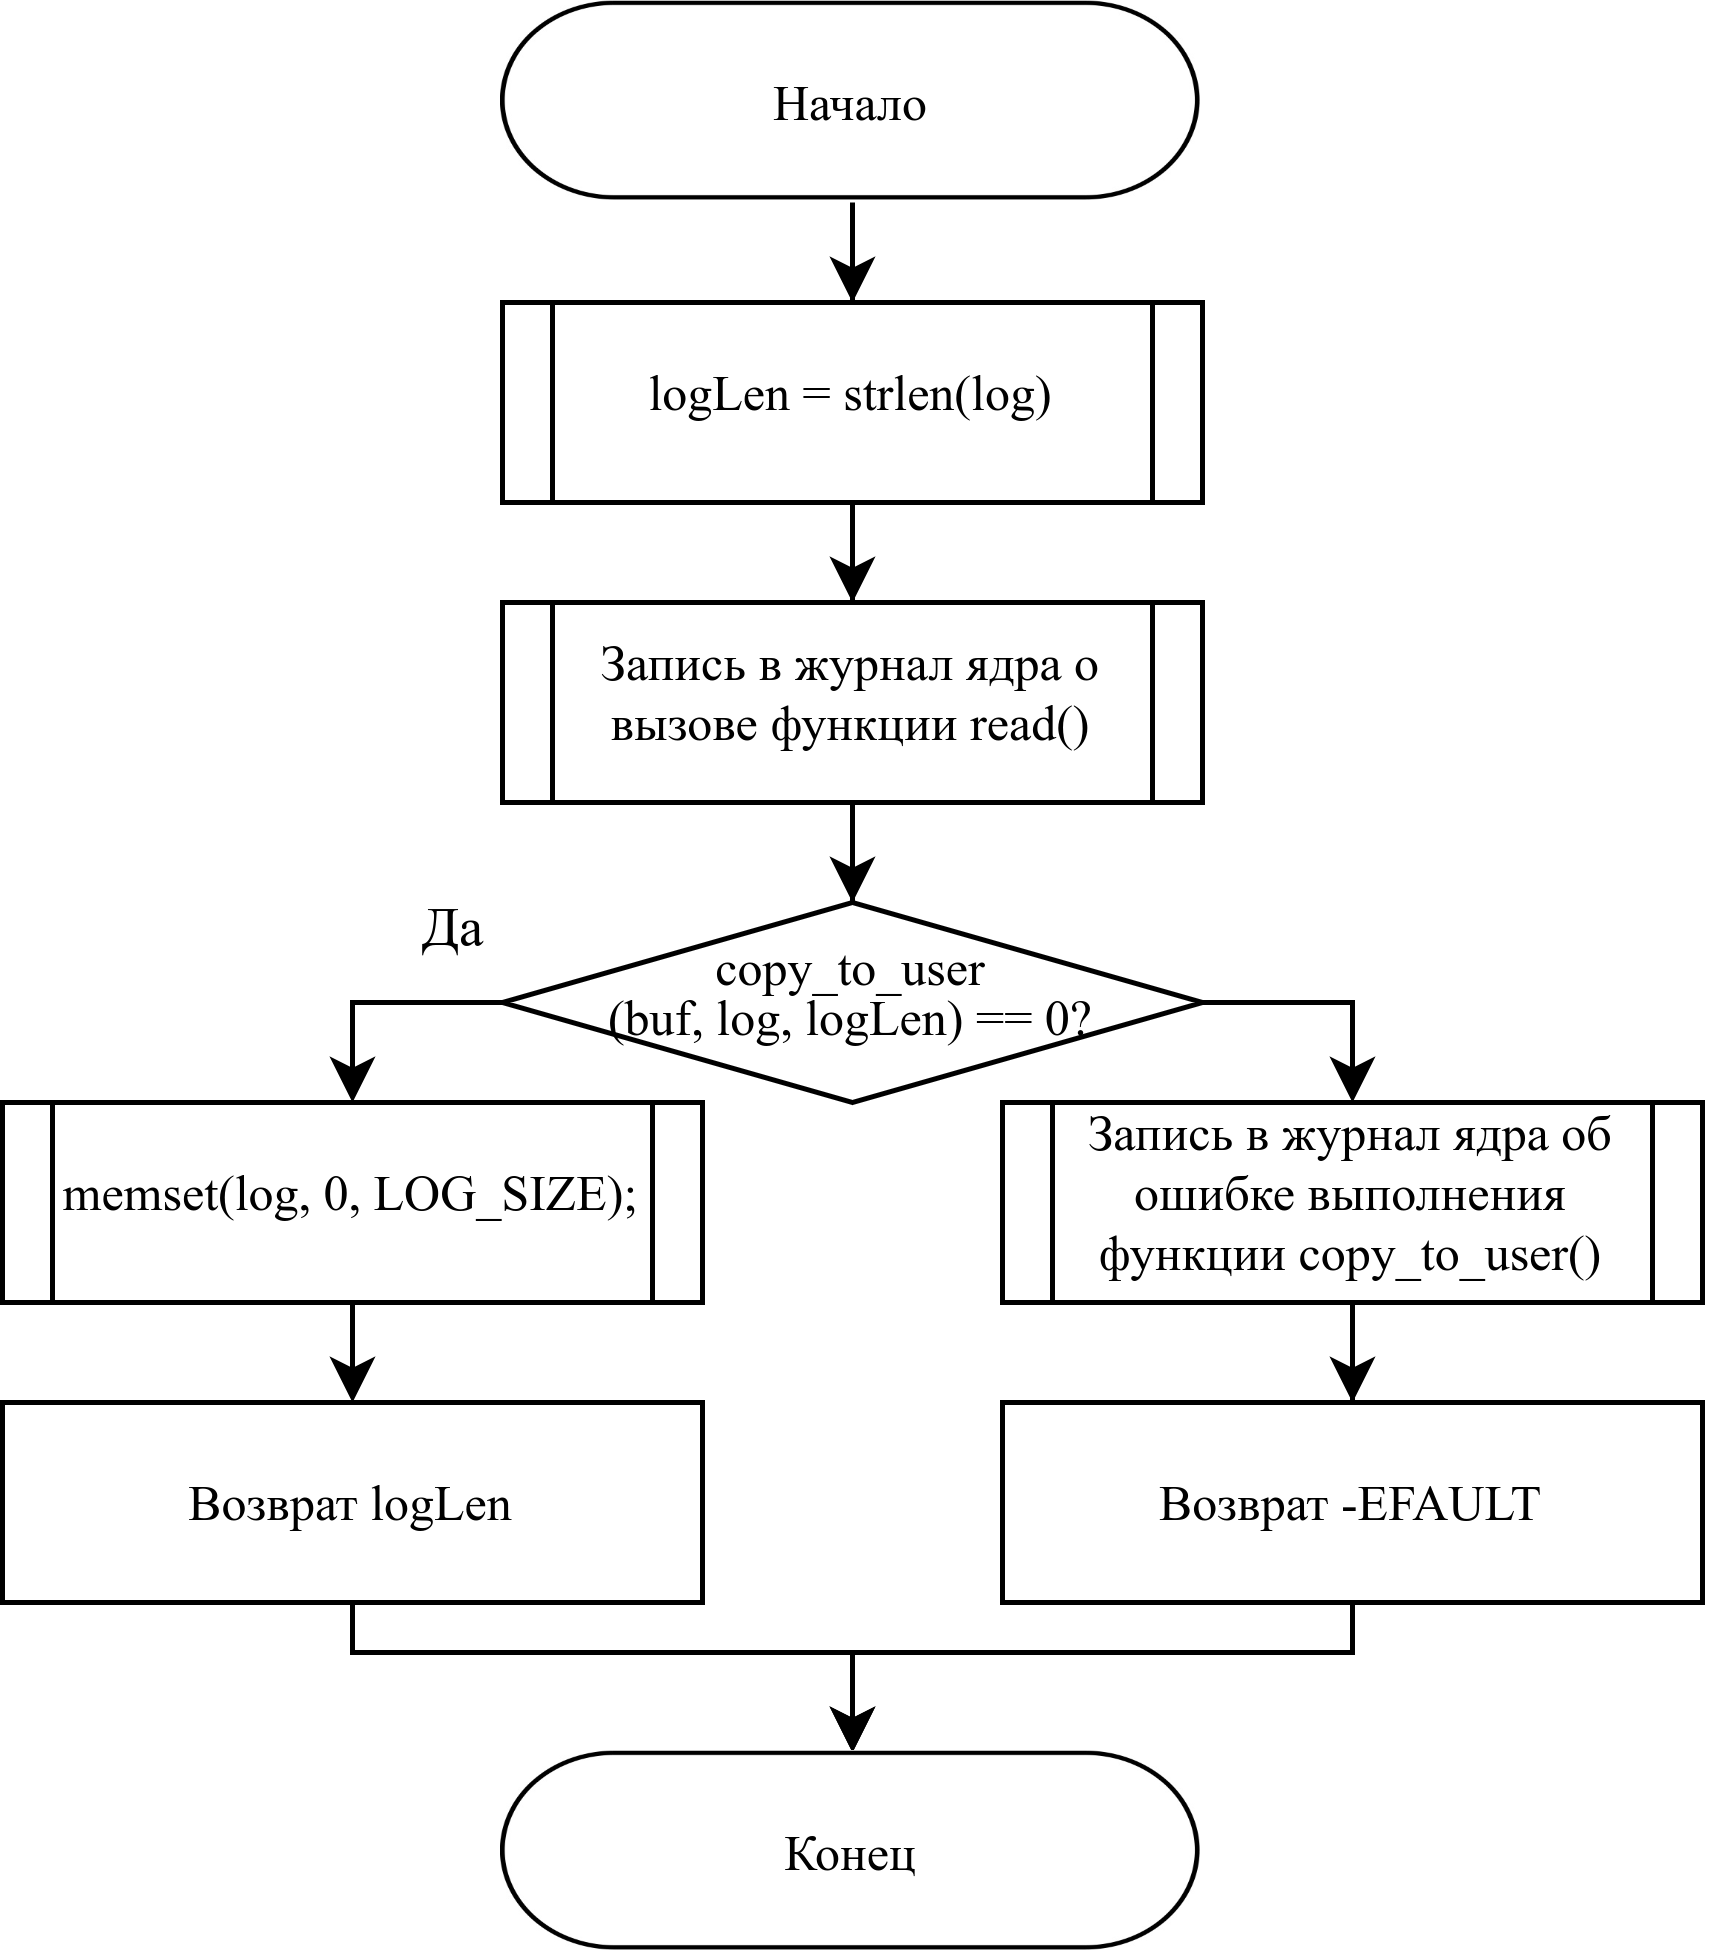
\includegraphics[scale=0.15]{assets/log.png}
	\caption{Алгоритм сохранения приоритетов, времени непрерывной работы, простоя и блокировки процессов}
	\label{fig:log}
\end{figure}

\section{Алгоритм предоставления информации о процессах пользователю}

На рисунке \ref{fig:user} представлен алгоритм предоставления информации об изменении приоритетов, времени непрерывной работы, простоя и блокировки процессов пользователю.

\begin{figure}[H]
	\centering
	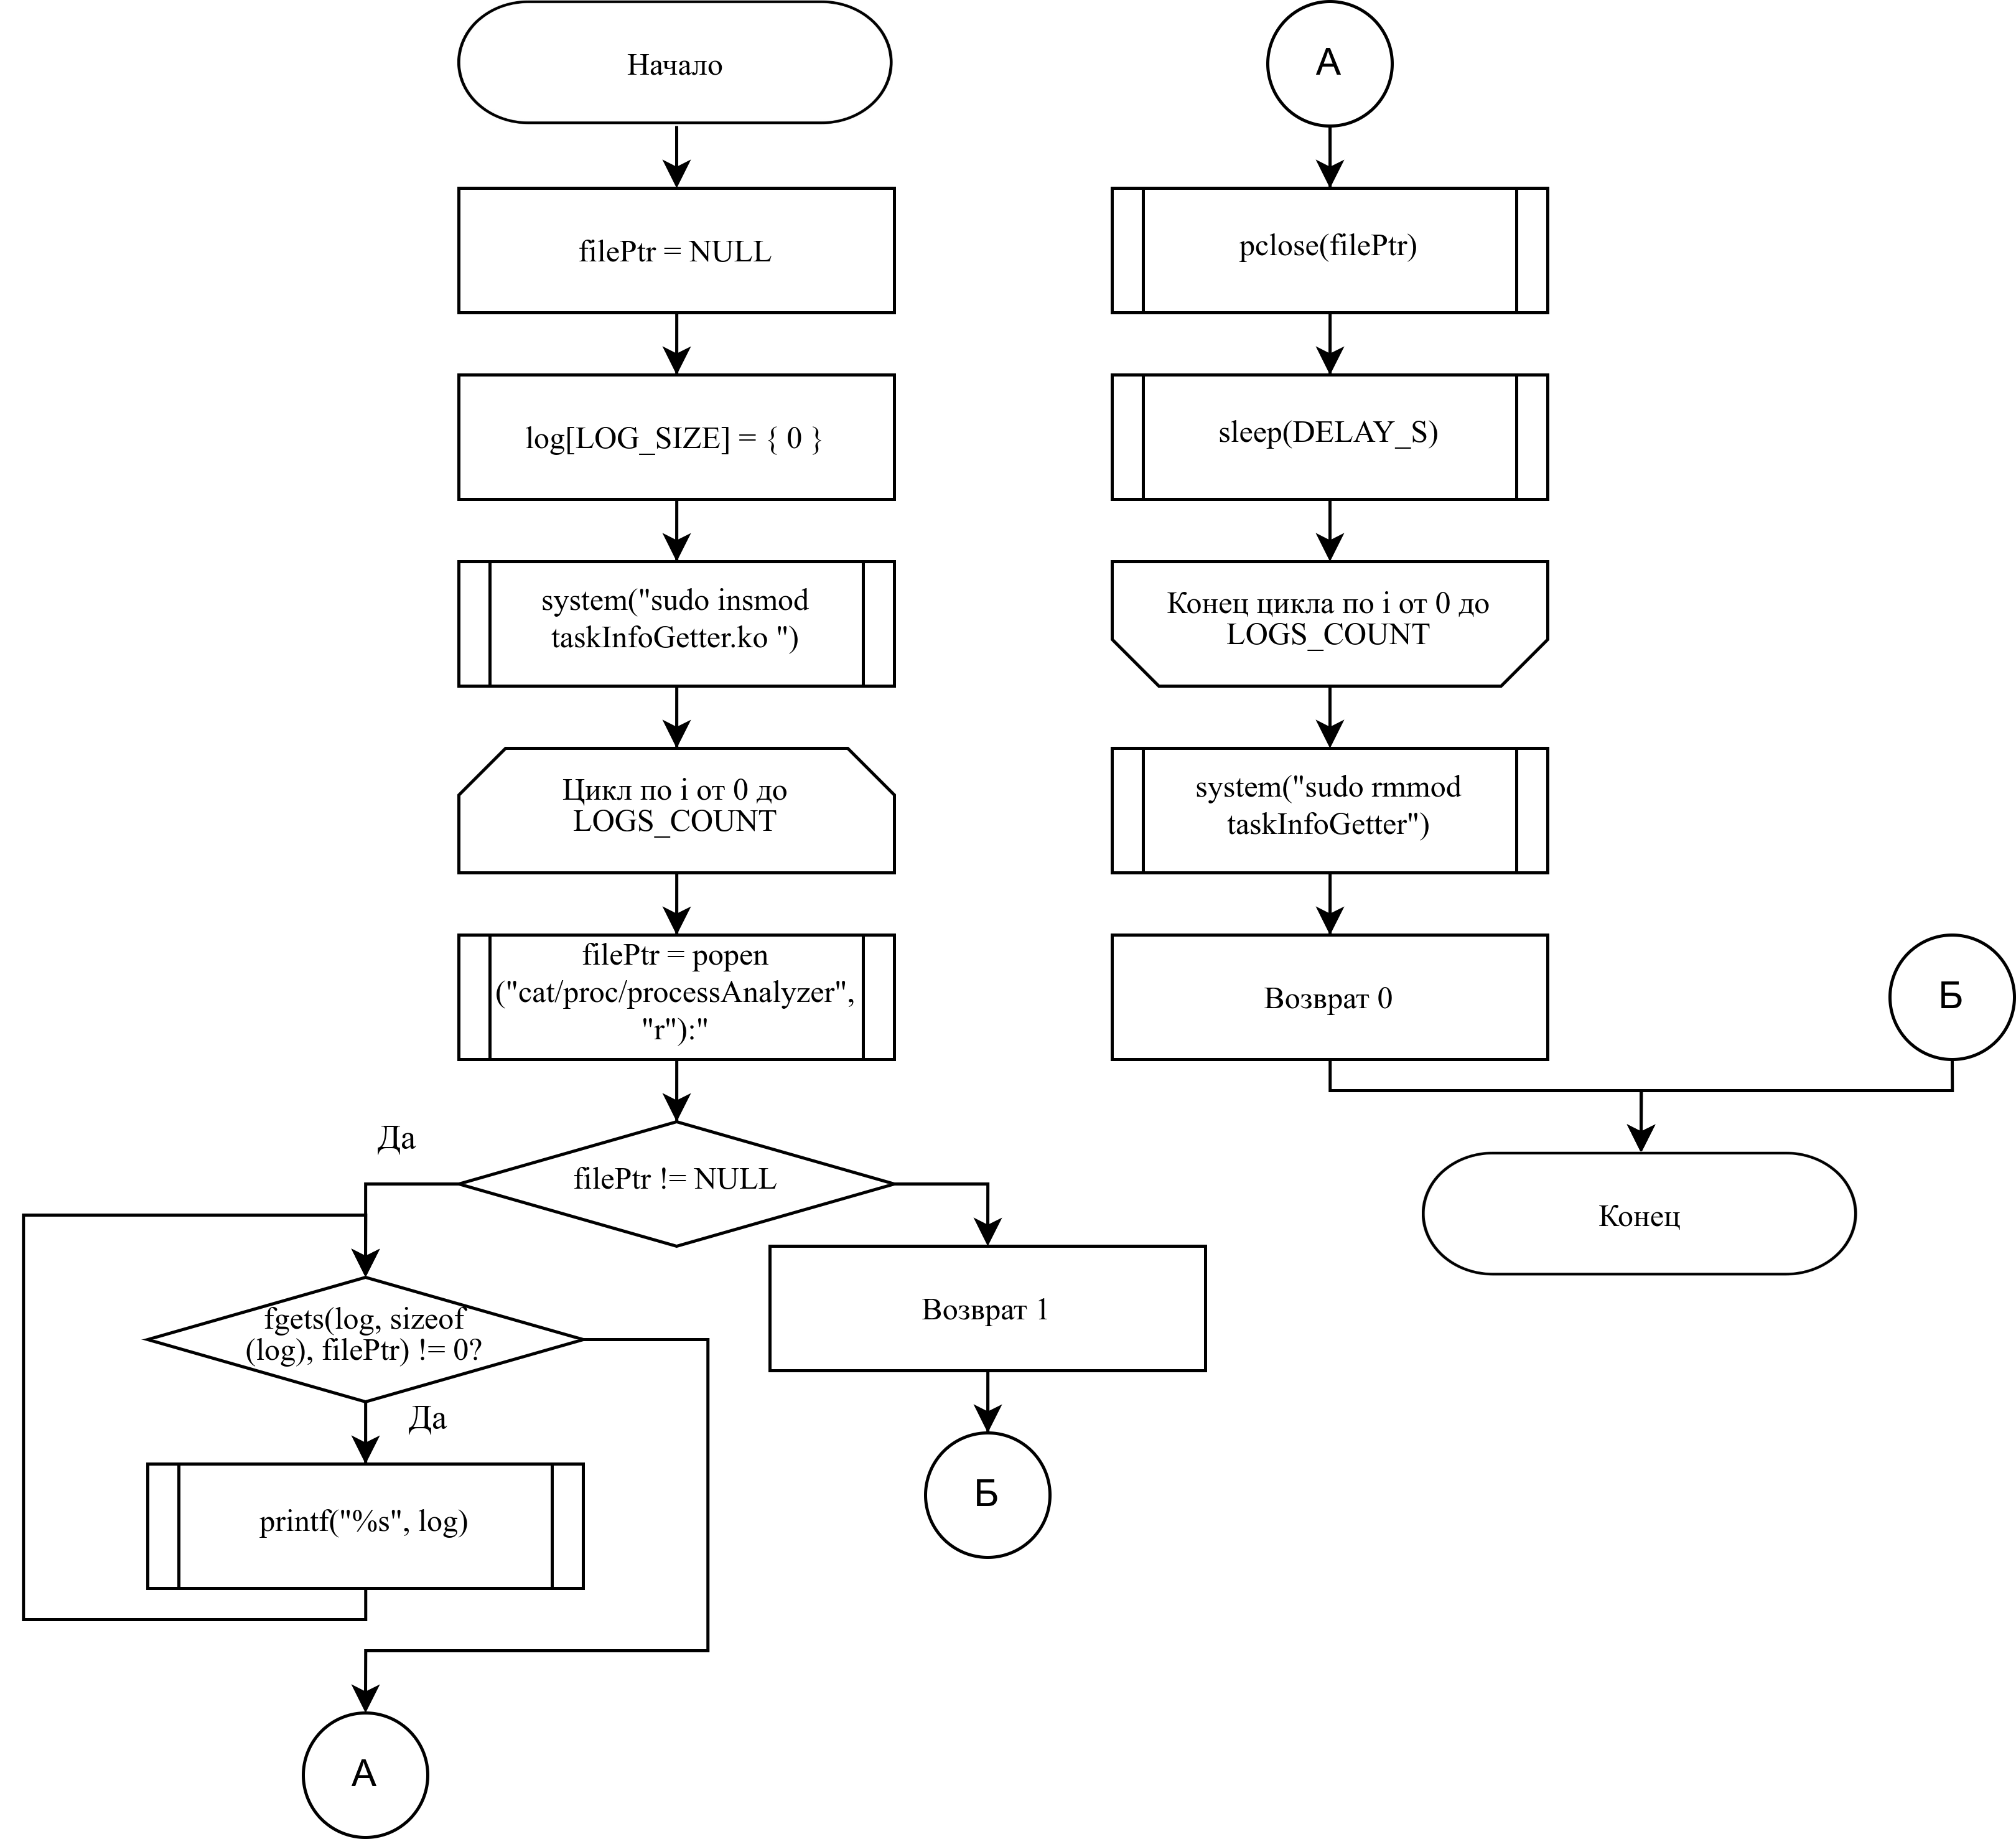
\includegraphics[width=\textwidth]{assets/user.png}
	\caption{Алгоритм предоставления информации об изменении приоритетов, времени непрерывной работы, простоя и блокировки процессов пользователю}
	\label{fig:user}
\end{figure}

\section{Структура программного обеспечения}

На рисунке \ref{fig:structure} представлена структура программного обеспечения.

\begin{figure}[H]
	\centering
	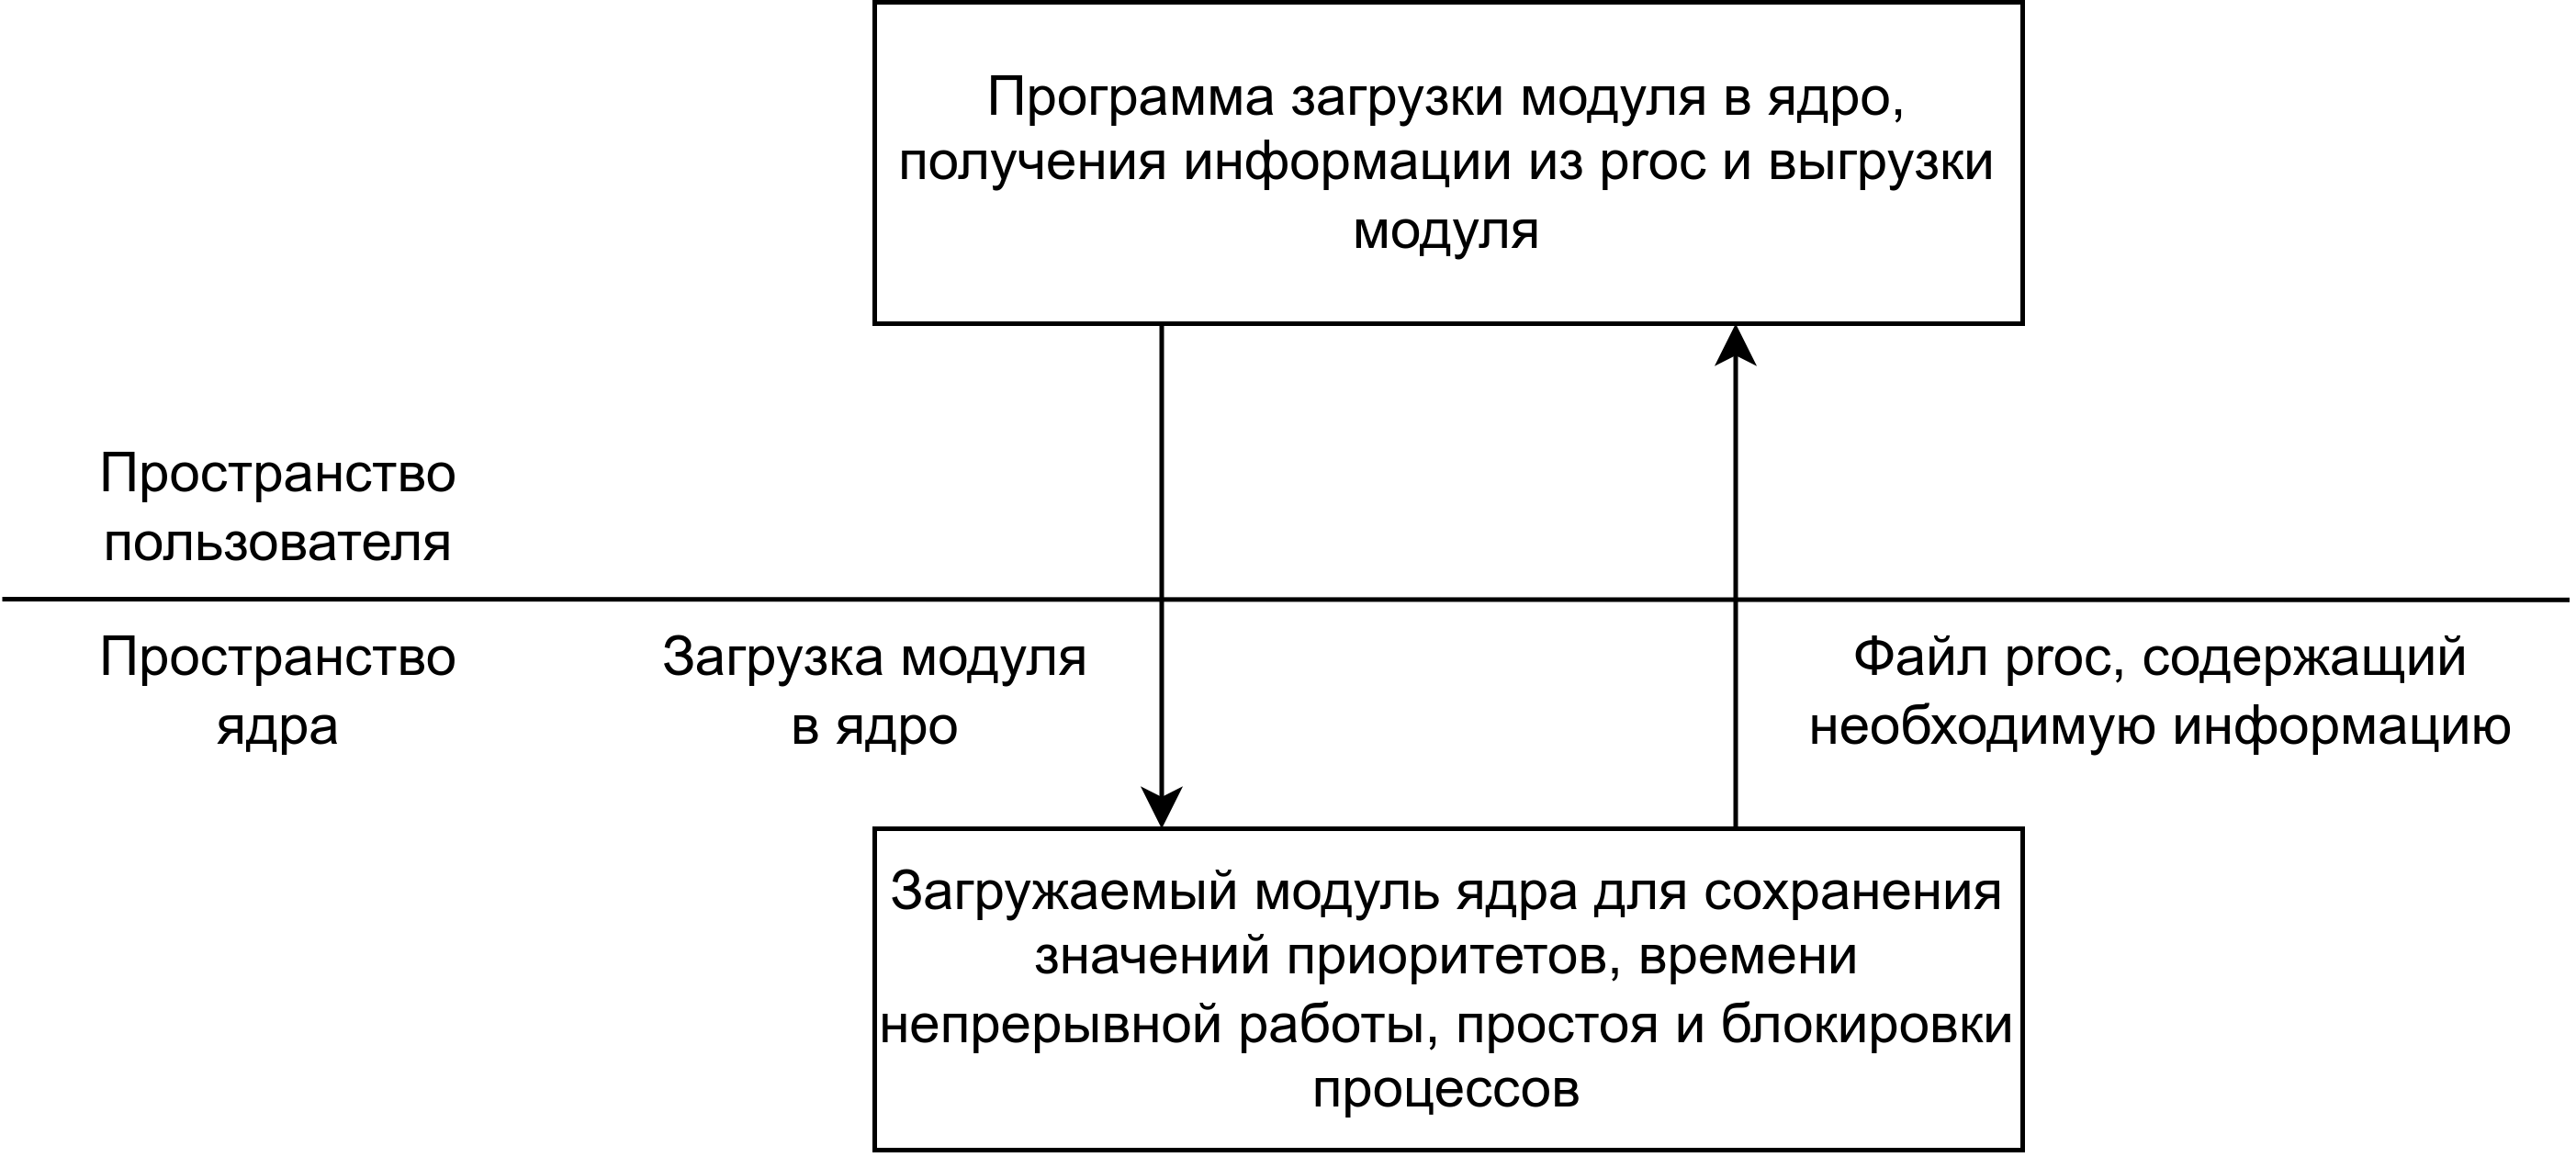
\includegraphics[width=\textwidth]{assets/structure.png}
	\caption{Структура программного обеспечения}
	\label{fig:structure}
\end{figure}


